\chapter{Probability on finite spaces}\label{ch:prob}
\index{probability}

Probability on finite spaces is Chapter~8's counting with a
denominator: $\#\text{good} / \#\text{all}$. The new content is what
happens when events interact --- conditioning, independence, and
expectation --- and the flagship result is that expected values add
even when the events do not. After this chapter you can model a random
experiment as a sample space, run conditional probabilities through a
tree, and use linearity of expectation where a direct count would be
hopeless.

\section{Sample spaces and uniform models}\label{sec:sample}
\index{sample space}
A sample space $\Omega$ is the set of all outcomes; an event is a
subset. Uniform model: every outcome equally likely, so
$P(A) = |A|/|\Omega|$ --- probability becomes combinatorics. The
uniformity must be \emph{verified} (``equally likely'' is a claim, not a
decoration): dealing cards uniformly is fine; summing two dice is not
uniform over the sums.

\section{Events, complements, ``at least one''}\label{sec:complement}
\index{complement rule}
$P(\overline{A}) = 1 - P(A)$. The complement move converts ``at least
one'' into ``none'', and ``none'' factorises
(Figure~\ref{fig:complement}): $P(\text{at least one hit}) =
1 - P(\text{all misses})$.

\begin{figure}[ht]\centering
% Figure: complement for "at least one" -- the outside of the union.
% Source for Figure~\ref{fig:complement}. TikZ only; regenerable by compiling main.tex.
\begin{tikzpicture}[
  lab/.style={font=\footnotesize\sffamily,text=slate},
]
\draw[draw=rulegray,fill=rulegray!8] (-0.4,-1.5) rectangle (4.4,1.7);
\draw[draw=ink,fill=accent!20] (1.3,0) circle (0.95);
\draw[draw=ink,fill=accent!20] (2.6,0) circle (0.95);
\node[lab] at (0.9,0) {$A_1$};
\node[lab] at (3.0,0) {$A_2$};
\node[lab] at (1.95,0.0) {$\cap$};
\node[lab] at (2.0,1.35) {$A_1 \cup A_2$ = at least one};
\node[lab] at (2.0,-1.1) {the white region outside both circles is ``none''};
\node[lab] at (2.0,-1.9) {$P(\text{at least one}) = 1 - P(\text{none})$
 --- and ``none'' factorises};
\end{tikzpicture}

\caption{``At least one'' as a complement. Notice the white region is
the only part counted --- and it factorises, which is why the
complement is the computable side.}
\label{fig:complement}
\end{figure}

\begin{example}\label{ex:birthday}
How many people until a shared birthday is more likely than not?
\par\smallskip
\textbf{Strategy.} Compute the complement ``all distinct'' --- it is a
falling product, easy to evaluate; the event itself is an awkward
union.
\par\smallskip
\begin{solution}
$P(\text{all distinct}) = \frac{365}{365}\cdot\frac{364}{365}\cdots
\frac{365-k+1}{365}$; at $k = 23$ this first dips below $1/2$
($\approx 0.493$), so the threshold is 23 people. The paradox is that
pair-counting, not person-counting, drives it: $\binom{23}{2} = 253$
pairs.
\end{solution}
\end{example}

\section{Conditional probability}\label{sec:cond}
\index{conditional probability}
\begin{definition}
$P(A \mid B) = \dfrac{P(A \cap B)}{P(B)}$ for $P(B) > 0$ ---
the sample space shrinks to $B$; the four-step method is: draw the
tree, compute the branch weights, take the intersection, divide.
\end{definition}

\begin{example}\label{ex:cond}
A prize draw first picks a tier --- gold with probability $1/4$,
plain $3/4$ --- then pays out with probability $1/2$ on gold, $1/6$ on
plain. Given that a prize was won, what is the chance it came from the
gold tier?
\par\smallskip
\textbf{Strategy.} Define the event algebra before touching numbers:
want $P(\text{gold} \mid \text{win})$; build the tree, weight each
leaf, then divide the gold-leaf weight by the win leaves' total
(Figure~\ref{fig:ptree}).
\par\smallskip
\begin{solution}
Leaves: gold-win $= \frac14\cdot\frac12 = \frac18$;
plain-win $= \frac34\cdot\frac16 = \frac18$; the other two leaves
(gold-lose $\frac18$, plain-lose $\frac58$) condition out --- they are
not wins. So $P(\text{gold}\mid\text{win}) = \frac{1/8}{1/8+1/8}
= \frac{1}{2}$: knowing a prize was won doubles the chance it was
gold, since plain pays out at only a third of gold's rate.
\end{solution}
\end{example}

\begin{figure}[ht]\centering
% Figure: two-stage probability tree (prize draw).
% Source for Figure~\ref{fig:ptree}. TikZ only; regenerable by compiling main.tex.
\begin{tikzpicture}[
  nd/.style={circle,draw=rulegray,minimum size=3mm,inner sep=0pt},
  lab/.style={font=\footnotesize\sffamily,text=slate},
  ed/.style={draw=rulegray},
  el/.style={font=\scriptsize,text=slate},
]
\node[nd] (r) at (0,0) {};
\node[nd] (a) at (1.8,0.9) {};
\node[nd] (b) at (1.8,-0.9) {};
\draw[ed] (r) -- (a) node[midway,above,el] {gold $1/4$};
\draw[ed] (r) -- (b) node[midway,below,el] {plain $3/4$};
\foreach \p/\n in {a/{c1,c2},b/{d1,d2}} {}
\node[nd] (c1) at (3.6,1.5) {}; \node[nd] (c2) at (3.6,0.4) {};
\node[nd] (d1) at (3.6,-0.4) {}; \node[nd] (d2) at (3.6,-1.5) {};
\draw[ed] (a)--(c1) node[midway,above,el] {win $1/2$};
\draw[ed] (a)--(c2) node[midway,below,el] {lose $1/2$};
\draw[ed] (b)--(d1) node[midway,above,el] {win $1/6$};
\draw[ed] (b)--(d2) node[midway,below,el] {lose $5/6$};
\node[lab] at (5.0,1.5) {$1/8$};
\node[lab] at (5.0,0.4) {$1/8$};
\node[lab] at (5.0,-0.4) {$1/8$};
\node[lab] at (5.0,-1.5) {$5/8$};
\node[lab] at (2.5,-2.3) {$P(\text{gold} \mid \text{win}) = \frac{1/8}{1/8+1/8} = \frac{1}{2}$};
\end{tikzpicture}

\caption{The four-step method on the prize draw. Notice the
conditioning just deletes leaves: the answer lives entirely inside the
win leaves' mass, and every leaf's weight is the product along its
path.}
\label{fig:ptree}
\end{figure}

\section{Independence, and when it fails}\label{sec:indep}
\index{independence}
$A$ and $B$ are independent iff $P(A\cap B) = P(A)P(B)$ ---
equivalently $P(A\mid B) = P(A)$. It is a property to \emph{prove},
not an assumption to reach for: two people sharing a birthday is
roughly independent of \emph{another} pair sharing, but within one
group the events collide. The test is always the product rule: does
knowing $B$ change $A$'s probability?

\begin{figure}[ht]\centering
\begin{tikzpicture}[x=2.4cm,y=1.7cm]
  \draw (0,0) grid (2,2);
  \node[font=\small] at (-0.4,1.5) {heads};
  \node[font=\small] at (-0.4,0.5) {tails};
  \node[font=\small] at (0.5,2.4) {heads};
  \node[font=\small] at (1.5,2.4) {tails};
  \foreach \x/\y in {0.5/1.5,1.5/1.5,0.5/0.5,1.5/0.5}
    \node[font=\small] at (\x,\y) {$1/4$};
  \node[font=\small,align=left,anchor=west] at (2.5,1) {every cell $= \tfrac12\cdot\tfrac12$: coin 2's outcome\\changes nothing about coin 1's probability};
\end{tikzpicture}

\caption{Two fair coins: the joint table factors cell-by-cell. Notice
independence is a \emph{factorisation} claim --- every entry is a
product of marginals, which is exactly what $P(A\cap B) = P(A)P(B)$
says.}
\label{fig:indepgrid}
\end{figure}

\begin{example}\label{ex:pairwise}
Toss two fair coins; let $A$ = ``first heads'', $B$ = ``second
heads'', $C$ = ``outcomes agree''. Show $A$, $B$, $C$ are
\emph{pairwise} independent yet not jointly independent.
\par\smallskip
\textbf{Strategy.} Check the definition literally: every pair must
factor, and the triple intersection must fail to factor.
\par\smallskip
\begin{solution}
$P(A) = P(B) = P(C) = 1/2$. Each pair's intersection is a single
outcome: $A \cap B = \{HH\}$, $A \cap C = \{HH\}$, $B \cap C =
\{HH\}$, each of probability $1/4 = (1/2)(1/2)$ --- pairwise
independence holds. But $A \cap B \cap C = \{HH\}$ has probability
$1/4 \neq 1/8 = P(A)P(B)P(C)$. Equivalently: knowing $A$ \emph{and}
$B$ determines $C$ exactly. Pairwise independence does not imply joint
independence --- the conjunction can carry information no single pair
reveals.
\end{solution}
\end{example}

\section{Random variables and expectation}\label{sec:rv}
\index{random variable}\index{expectation}
A random variable is a function $X : \Omega \to \mathbb{R}$;
$E[X] = \sum_\omega X(\omega)\,P(\omega)$. The definition is
deceptively plain --- its power is in the next section's linearity.

\begin{figure}[ht]\centering
\begin{tikzpicture}[x=1.1cm,y=0.9cm]
  % PMF of fair die, E as fulcrum
  \foreach \x/\h in {1/1,2/1,3/1,4/1,5/1,6/1}{
    \draw[fill=accent!25] (\x-0.3,0) rectangle (\x+0.3,\h);
    \node[font=\small] at (\x,-0.5) {\x};
  }
  \draw[->] (0,0) -- (7,0);
  \draw[->] (0,0) -- (0,1.8);
  \node[font=\small,left] at (0,1) {$1/6$};
  % fulcrum at 3.5
  \draw[fill=ink] (3.5,-0.25) -- (3.2,-1.1) -- (3.8,-1.1) -- cycle;
  \node[font=\small] at (3.5,-1.5) {$E[X] = 3.5$};
\end{tikzpicture}

\caption{Expectation as a balance point: the pmf of a fair die balances
at $3.5$. Notice $E[X]$ need not be a value $X$ ever takes --- it is a
centre of mass, not a prediction.}
\label{fig:exbalance}
\end{figure}

\section{Linearity of expectation}\label{sec:linexp}
\index{linearity of expectation}
\begin{theorem}
$E[X_1 + X_2 + \cdots + X_n] = E[X_1] + \cdots + E[X_n]$
--- always, with no independence hypothesis.
\end{theorem}

\begin{example}\label{ex:fixpts}
Find the expected number of fixed points of a random permutation of
$n$ elements.
\par\smallskip
\textbf{Strategy.} Do not count the distribution --- it depends
horribly on $n$. Write $X = \sum_i \mathbb{1}\{\sigma(i) = i\}$;
each indicator has $E = 1/n$ (position $i$ is fixed with probability
$1/n$), and linearity needs nothing else (Figure~\ref{fig:indicator}).
\par\smallskip
\begin{solution}
$E[X] = \sum_{i=1}^{n} \frac{1}{n} = 1$, for every $n$ --- exact, and
Listing~\ref{lst:fixpts} confirms it empirically.
\end{solution}
\end{example}

\begin{figure}[ht]\centering
% Figure: fixed-point indicator table for permutations of 4 (compact).
% Source for Figure~\ref{fig:indicator}. TikZ only; regenerable by compiling main.tex.
\begin{tikzpicture}[
  lab/.style={font=\footnotesize\sffamily,text=slate},
  hd/.style={font=\footnotesize\bfseries},
  cell/.style={font=\scriptsize},
]
% 4x4 header + a few rows of the 24
\node[hd] at (0,0.7) {$\sigma$};
\node[hd] at (0.9,0.7) {$\mathbb{1}_1$};
\node[hd] at (1.6,0.7) {$\mathbb{1}_2$};
\node[hd] at (2.3,0.7) {$\mathbb{1}_3$};
\node[hd] at (3.0,0.7) {$\mathbb{1}_4$};
\node[hd] at (3.9,0.7) {$X$};
\foreach \r/\s/\a/\b/\c/\dd/\x in {
  0/{1234}/1/1/1/1/4,
  1/{1243}/1/1/0/0/2,
  2/{1324}/1/0/1/0/2,
  3/{2143}/0/0/0/0/0,
  4/{4321}/0/0/0/0/0
}
{
  \node[cell] at (0,{0.3-\r*0.4}) {\s};
  \node[cell] at (0.9,{0.3-\r*0.4}) {\a};
  \node[cell] at (1.6,{0.3-\r*0.4}) {\b};
  \node[cell] at (2.3,{0.3-\r*0.4}) {\c};
  \node[cell] at (3.0,{0.3-\r*0.4}) {\dd};
  \node[cell] at (3.9,{0.3-\r*0.4}) {\x};
}
\node[lab] at (0.5,-1.9) {$\vdots$ 24 rows};
\node[lab] at (2.0,-2.5) {column sums: each $\mathbb{1}_i$ totals $3! = 6$; $\sum X = 4 \cdot 6 = 24$; $E[X] = 24/24 = 1$};
\end{tikzpicture}

\caption{The indicator table idea ($n = 4$ shown compactly). Notice the
proof is a column count: each $\mathbb{1}_i$ column sums to $3!$ over
the $4!$ rows --- the indicators are nowhere near independent, and
linearity does not care.}
\label{fig:indicator}
\end{figure}

\begin{checkpoint}[Predict before you run]
Listing~\ref{lst:fixpts} simulates permutations of $6$ for $10{,}000$
trials. Predict the estimate to two decimals before reading the output
--- and the size of the residual.
\end{checkpoint}

\begin{lstlisting}[language=Python,caption={\texttt{fixed\_points.py}:
Monte Carlo vs exact theory (script in
\texttt{code/fixed\_points.py}).},label={lst:fixpts}]
total += sum(p[i] == i for i in range(n))
\end{lstlisting}
Real output:
\begin{lstlisting}[numbers=none]
permutations of n = 6, 10000 Monte Carlo trials
estimated E[fixed points] = 1.0048
exact value               = 1 (n * 1/n, linearity of expectation)
relative error            = 0.48%
\end{lstlisting}

\section{Simpson's paradox}\label{sec:simpson}
\index{Simpson's paradox}

\begin{example}\label{ex:simpson}
Drug A beats drug B separately among mild and severe cases, yet loses
overall --- construct the table.
\par\smallskip
\textbf{Strategy.} Weighted sums on a $2\times2\times2$ table: rates
can win per stratum and still lose when the groups' sizes skew the
mixture. Arithmetic, not opinion.
\par\smallskip
\begin{solution}
A wins both strata --- mild: $80/100 = .80$ vs B's $79/100 = .79$;
severe: $20/100 = .20$ vs B's $5/50 = .10$ --- yet loses the pool:
A $= 100/200 = .50$ against B $= 84/150 = .56$. The trick is the mix:
B's patients were mostly mild, where everyone's rate is high, so B's
pooled rate rides the mild stratum's weight. Weighted means move with
the weights --- that is the whole paradox.
\end{solution}
\end{example}

\section{Geometric probability preview}\label{sec:geo}
\index{geometric probability}
When the space is continuous, counts become areas or volumes:
a uniform point in the unit square hits the quarter-circle
with probability $\pi/4$ (Figure~\ref{fig:geo}) --- the same
``favourable/total'' shape, measured instead of counted. The discrete
habits (conditioning, complements, indicators) all carry over.

\begin{figure}[ht]\centering
% Figure: geometric probability -- quarter-circle in a unit square.
% Source for Figure~\ref{fig:geo}. TikZ only; regenerable by compiling main.tex.
\begin{tikzpicture}[
  lab/.style={font=\footnotesize\sffamily,text=slate},
]
\draw[draw=ink] (0,0) rectangle (3,3);
\draw[draw=accent,very thick,fill=accent!15] (0,0) -- (3,0) arc (0:90:3) -- cycle;
\node[lab] at (0.7,0.9) {hit};
\node[lab] at (2.2,2.5) {miss};
\node[lab] at (1.5,-0.5) {unit square, quarter-circle of radius 1};
\node[lab] at (1.5,-1.0) {$P(\text{hit}) = \dfrac{\pi/4}{1} = \dfrac{\pi}{4}$
 --- areas replace counts};
\end{tikzpicture}

\caption{Geometric probability: the region's \emph{area} replaces the
count. Notice nothing else changes --- favourable over total, just
measured.}
\label{fig:geo}
\end{figure}

\begin{exercise}[easy]\label{exr:p1}
Two dice: $P(\text{sum} = 7)$? Explain why $1/11$ is wrong and what
the sample space actually is.
\end{exercise}
\begin{exercise}[medium]\label{exr:p2}
Three fair coin flips: find $P(\text{at least one head})$ by
complement, then the probability of exactly one head.
\end{exercise}
\begin{exercise}[medium]\label{exr:p3}
Expected number of aces in a 5-card hand --- by indicators, not by the
hypergeometric formula.
\end{exercise}
\begin{exercise}[medium]\label{exr:p4}
A test is $99\%$ accurate on a disease with prevalence $1/1000$.
Compute $P(\text{disease} \mid \text{positive})$ --- the prosecutor's
fallacy gap.
\end{exercise}

\section{Chapter summary}
\begin{table}[ht]\centering
\begin{tabularx}{\linewidth}{@{}lYY@{}}
\toprule
\tablehead\thead{Tool} & \thead{Formula} & \thead{When}\\
\midrule
uniform count & $|A|/|\Omega|$ & verify uniformity first\\
complement & $1 - P(\overline{A})$ & ``at least one''\\
conditioning & $P(A\cap B)/P(B)$ & tree + four steps\\
independence & $P(A)P(B)$ & prove it, don't assume\\
linearity & $\sum E[\mathbb{1}_i]$ & indicators, always\\
geometric & area ratio & continuous spaces\\
\bottomrule
\end{tabularx}
\caption{One page: counting with a denominator, plus the three rules
that survive when events interact.}
\label{tab:prob}
\end{table}

\section{Common mistakes}
\index{common mistakes}
\begin{itemize}
\item \textbf{Assuming independence.} ``Looks unrelated'' is not a
proof; the product rule is a theorem-level claim that must be verified.
The birthday paradox is exactly the price of assuming it.
\item \textbf{Adding where complements apply.} $P(A \cup B)$ is not
$P(A) + P(B)$ in general --- that is Chapter~9's PIE correction again;
``at least one'' wants $1 - P(\text{none})$.
\item \textbf{Flipping the condition.} $P(A\mid B) \ne P(B\mid A)$:
$P(\text{positive}\mid\text{disease}) = .99$ says nothing about
$P(\text{disease}\mid\text{positive}) \approx .09$ at $1/1000$
prevalence --- the prosecutor's fallacy, and it is arithmetic, not
intuition.
\end{itemize}

\section{Additional exercises}
\begin{exercise}[easy]
$P(\text{both heads})$ in two fair flips; then
$P(\text{both heads} \mid \text{at least one head})$. Same event ---
different space.
\end{exercise}
\begin{exercise}[easy]
Expected value of a fair die; then $E[X^2]$ and check that
$E[X^2] \ne (E[X])^2$ --- what does the gap measure?
\end{exercise}
\begin{exercise}[easy]
Draw four without replacement from $\{1,\dots,10\}$; find
the probability all are even.
\end{exercise}
\begin{exercise}[easy]
Rolls of two dice: is ``sum 7'' independent of ``first die 3''? Check
by the product rule, not by feel.
\end{exercise}
\begin{exercise}[medium]
Expected number of runs (maximal same-face blocks) in $n$ fair flips,
via indicators on the boundaries.
\end{exercise}
\begin{exercise}[medium]
Coupon collector for $n = 3$: expected draws to see all three types
--- split into geometric phases and add.
\end{exercise}
\begin{exercise}[medium]
Three prisoners and the jailer's reveal: compute
$P(\text{spared} \mid \text{jailer names a prisoner})$ --- where does
the naive $1/2$ go wrong?
\end{exercise}
\begin{exercise}[medium]
Derive the birthday threshold estimate $k \approx \sqrt{2 \cdot 365
\log 2}$ from the product formula (take logs, approximate
$\log(1-x) \approx -x$).
\end{exercise}
\begin{exercise}[medium]
Expected number of inversions in a random permutation of $n$ ---
indicators on pairs.
\end{exercise}
\begin{exercise}[hard]
Prove $\operatorname{Var}(X) = E[X^2] - (E[X])^2$ and compute the
variance of the fixed-point count (hint: indicators plus pairwise
products).
\end{exercise}
\begin{exercise}[hard]
Simpson's paradox: give a $2\times2\times2$ table where A wins both
strata by $\ge 10$ points but loses overall by $\ge 5$, and prove the
sizes must be skewed for this to happen.
\end{exercise}
\begin{exercise}[hard]
Extend \texttt{fixed\_points.py} to track the empirical \emph{maximum}
fixed-point count per trial over growing $n$ and describe the
maximum's behavior (conjecture: bounded in distribution with a slowly
growing tail --- collect data and state what you actually see).
\end{exercise}
\begin{exercise}[easy]
Two dice: find $P(\text{sum} = 7 \mid \text{first die} \ge 4)$.
\end{exercise}
\begin{exercise}[medium]
Show that if $A$ and $B$ are independent, so are $A$ and $B^c$ ---
independence survives complements (one line of algebra, not intuition).
\end{exercise}
\begin{exercise}[hard]
$100$ fair coins are flipped; find the expected number of runs of
$k = 3$ consecutive heads by linearity, then verify against
\texttt{fixed\_points.py}-style simulation.
\end{exercise}

\section*{Further reading}
\begin{itemize}
\item J.~Blitzstein and J.~Hwang, \emph{Introduction to Probability}
(free online edition) ---
\url{https://probabilitybook.net} --- the Stat 110 text; story-based
probability at exactly this chapter's level.
\item MIT OpenCourseWare, \emph{6.042J} (Fall 2010) ---
\url{https://ocw.mit.edu/6-042JF10} --- probability for CS; discrete,
combinatorial, no measure theory.
\item E.~Lehman, F.~T.~Leighton, A.~R.~Meyer, \emph{Mathematics for
Computer Science}, probability chapters ---
\url{https://courses.csail.mit.edu/6.042/spring18/mcs.pdf} --- free PDF;
linearity of expectation with combinatorial applications.
\item Berkeley CS70 notes ---
\url{https://www.eecs70.org/} --- free lecture notes; discrete
probability, conditioning and the birthday paradox.
\item E.~Chen, \emph{Expected Uses of Probability} ---
\url{https://web.evanchen.cc/handouts/ProbabilisticMethod/ProbabilisticMethod.pdf}
--- olympiad linearity tricks and the probabilistic method.
\item R.~Hammack, \emph{Book of Proof}, 3rd ed. ---
\url{https://richardhammack.github.io/BookOfProof/} --- for tightening
the probabilistic-argument writing style.
\end{itemize}

\begin{rulebox}[Watch instead]
\begin{itemize}
\item \textbf{Harvard Stat 110 --- ``Lecture 1: Probability and
Counting'' (Joe Blitzstein)}, 46:29,
\url{https://www.youtube.com/watch?v=KbB0FjPg0mw} --- sample spaces and
the naive definition, exactly the tone of \S\ref{sec:sample}--%
\S\ref{sec:complement}. (Verified 2026-10-11.)
\item \textbf{Harvard Stat 110 full playlist (Blitzstein)}, 34
lectures,
\url{https://www.youtube.com/playlist?list=PLLVplP8OIVc8EktkrD3Q8td0GmId7DjW0}
--- the entire free course this chapter previews.
(Verified 2026-10-11.)
\end{itemize}
\end{rulebox}

\chapternotes
The four-step method, tree diagrams, linearity of expectation and the
Simpson's-paradox setup follow 6.042J's probability
chapters~\cite{mcs}; Berkeley CS70's probability note sequence carries
the same material with more rigor~\cite{cs70}; Chen's \emph{Expected
Uses of Probability} supplies the indicator-table worked
pattern~\cite{chen-expected}, and Zhao's counting-adjacent handouts the
olympiad drills~\cite{zhao}. Contest items powered by this chapter ---
conditional probability and trees (AIME 2024 I P4, AIME 2023 I P6,
AIME 2021 I P1, AIME 2015 I P2), expectation by linearity (AIME 2024 I
P11, AIME 2021 I P12, AIME 2018 I P12, AIME 2023 II P6), complements
and birthdays (AIME 2023 I P1, AIME 2020 I P9, AIME 2018 I P3, AIME
2015 I P5), plus AMC items (AMC 12 2023 A P5, AMC 12 2023 A P17, AMC
12 2024 A P16, AMC 12 2024 A P20, AMC 12 2024 B P9, AMC 12 2024 B
P17, AIME 2010 I P1, AIME 2010 I P4, AIME 2025 II P7) --- are on the
AoPS archive~\cite{aops-amc}.
